\section{Параллельная версия метода}
\subsection{Необходимость}
Однопроцессорная версия алгоритма имеет весьма ограниченную применимость: основным лимитирующим фактором является объём оперативной памяти, доступной на локальном вычислительном узле. Границы применимости однопроцессорной версии можно получить при помощи следующих предположений:
\begin{itemize}
	\item используемые типы данных -- float (4 байта) и int (4 байта);
	\item в каждом узле сетки хранится 3 значения вектора скорости, 6 значений тензора, по 3 значения координат в локальной и подвижной системах, 4 значения параметров реологии среды;
	\item в процессе расчёта каждого временного шага требуется хранить копию расчётов предыдущего временного слоя, для записи результатов на жёсткий диск необходима третья копия;
	\item каждый узел хранит информацию о <<локальной>> топологии сетки для быстрого доступа к соседним тетраэдрам и треугольникам (в среднем по пять значений типа int для каждого типа элементов).
\end{itemize}

Суммарно имеем следующий расход памяти на хранения одного узна: 228 байт. В этих расчётах не учитываются расходы на хранения топологии всей сетки, в виду сложности проведения оценки. Таким образом получаем, что при доступном объёме памяти в 1 Гб для одного вычислительного узла с максимальной скоростью можно проводить расчёты на сетках с числом узлов \todo{Эта цифра немного не сходится с расчётами выше}1-2 миллиона. Под максимальной скоростью здесь понимается следующее: при расчёте на сетках указанного выше размера все необходимые данные могут быть полностью помещены в оперативной памяти, скорость доступ к которой на порядки выще скорости чтения с жёсткого диска.

Характерный размер сетки для решаемый задачи — \todo{Посчитать объём точнее} 792000 узлов (11 слоёв, каждый из которых имеет размер 120x120x5). Стоит отдельно отметить, что размеры этой задачи лежат на самой нижней границе характерных размеров задач, решение которых представляет практический интерес. Поставленную задачу уже весьма проблематично решить на одном вычислительном узле ввиду ограниченного размера доступной для вычислений оперативной памяти.

Другой причиной необходимости создания параллельной версии алгоритма является характер роста вычислительной сложности при увеличении числа узлов сетки ($O(n^3)$). Отсюда следует, что при уменьшении характерных размеров задачи вдвое сложность вычислений возрастает в 8 раз. Очевидно, что задачи такого класса необходимо решать при помощи параллельных версий алгоритмов, чтобы обеспечить хотя бы небольшую масштабируемость.

Таким образом создание параллельной версии алгоритма становится необходимым условием численного моделирования задач подобного рода.

\subsection{Способ построения параллельной версии}
Для реализации параллельных вычислений исходная геометрия разбивается на зоны, которые распределяются между вычислительными узлами. Один узел может производить одновременный расчёт нескольких зон. Для обеспечения согласованности расчёта вычислительные узлы обмениваются необходимой информацией о значениях и топологии сеток на границах зон. Для получения максимальной эффективности при параллельном расчёте следует учитывать следующие условия:
\begin{itemize}
	\item для увеличения времени полезного использования кластера необходимо, чтобы время расчёта очередного временного слоя на каждом вычислительном узле было примерно одинаково, так как в противном случае наиболее <<быстрые>> узлы проводят некоторые время в ожидании, при этом не проводя никаких расчётов;
	\item для увеличения скорости синхронизации и расчёта контактынх границ крайне желательно, чтобы зоны имели простую геометрию;
	\item граничные части сеток различных зон должны быть построены согласованно (в идеале должны совпадать топологически) для уменьшения потерь точности, связанных с интерполяцией;
	\item расчёт каждого временного слоя должен быть максимально <<параллельным>> в том смысле, что синхронизации происходят редко и согласованно, а данные передаются большими объёмами.
\end{itemize}
\subsubsection{Тестрирования производительности MPI}
Для выбора правильных API для построения параллельной версии был проведён ряд тестов производительности обмена сообщениями при помощи MPI. Одним из наиболее важных вопросов, ответ на которых хотелось получить был следующий: каков оптимальный объём сообщения для пересылки? Иными словами, нужно было выяснить, при каких размерах посылаемого сообщения время, затрачиваемое на пересылку одного байта, минимально.
Ниже приведены графики зависимости затрат на пересылку одно байта в зависимости от размера сообщения.
\begin{figure}[htp]
\centering
\includegraphics[width=0.8\textwidth]{eps/mpi-1host.eps}
\caption{Затраты на пересылки при использовании одного вычислительного
 узла}
\label{pic:mpi1host}
\end{figure}
\begin{figure}[htp]
\centering
\includegraphics[width=0.8\textwidth]{eps/mpi-2hosts.eps}
\caption{Затраты на пересылки при использовании двух вычислительных узлов}
\label{pic:mpi2hosts}
\end{figure}
Как видно из графиков, для пересылки данных посредство MPI выгодно использовать большие объёмы сообщений. В первую очередь это связано с сильным ростом накладных расходами на пересылку сообщения при уменьшении его размера. Другими фактороми, снижающими скорость передачи, могут служить буферизация исходящих сообщения, а также блокировки вызывающего процесса при синхронной передаче данных. По результатам проведённых тестов были сделаны следуюшщие выводы;
\begin{itemize}
	\item данные нужно передавать большими объёмами, так скорость в таких случаях выше;
	\item следует использовать асинхронную передачу данных, возможно, с инициацией приёма до момента послки данных;
	\item для ускорения процесса синхронизации крайне желательно использовать <<родные>> функции коллективного обмена данными вместо самостоятельной реализации подобного функционала;
	\item следует в полной мере использовать возможности MPI по созданию пользовательских типов данных для уменьшения объёмов памяти, требуемых для хранения временных структур данных, а также для уменьшения временн\'{ы}х затрат на копирование данных внутри вычислительного узла.
\end{itemize}

\subsubsection{Синхронизация шага по времени}
\subsubsection{Синхронизация узлов}
\subsubsection{Детектор столкновений}
\subsubsection{Синхронизация тетраэдров}
\subsubsection{Производительность параллельной версии}
